Conventional synchronous machines were found not to be able to ensure transient frequency stability in conditions of power imbalance exceeding 2\% in the case of the European model. The governor operation is by far too slow to constitute the unique solution for frequency support during the transient period. Inverter based fast power reserve would be needed to be activated in an extreme short time. Some extended capability to withstand power imbalances is observed with the faster governor response in the IEEE models. \\

Although unlikely to occur, the consideration of the uncertainty of synchronous reserves availability and possible power transmission congestion in future scenarios[], could lead to higher imbalances as nowadays. In order to avoid load shedding in penetration scenarios above 80\% of non-synchronous generation for and load imbalances up to 40\%, inverter based fast power reserve must be deployed over a time in the order of 100-500 ms, independently of grid size and primary reserve response. Nevertheless, today’s full power activation time of renewable sources without storage is in the range of 200 to 600 ms \footnote{Times required for the all measurement, signal transmission and processing and coordination of power electronic device's controls [ref]}. These activation times are adequate for power imbalances leading to values of RoCoF equal or less than 4 Hz/s as studied by ENTSOE in future scenarios [ref]. Hence with today’s frequency measuring time and power deployment from renewable sources; load shedding and possible total black outs would not be avoided. In scenarios with plenty of renewables and high expected imbalances, storage would be a key factor in order to avoid de-loading and curtailment of renewables, the fast activation times (<50 ms) and promising price reduction make storage a good strategy to provide power balancing in both over and under frequency cases [ref]. A comprehensive method for the estimation of the required time for the activation of the inverter based reserve was developed in this paper, with such method a frequency support strategy for inverters can be implemented for an expected level of imbalance as long as system inertia is monitored or estimated.\\

Synthetic inertia from wind turbines have a better performance when operated along with fast synchronous response systems as shown in section \ref{sec:res_si} with the simplified IEEE model. When synthetic inertia is implemented with slower response primary response such the case of the large scale of the European grid, it was not noted an appreciable improvement in regards of the frequency nadir. Therefore, synthetic inertia is not able by it self to regulate or restore frequency deviation[ref]. This predictable outcome limits its usage just for slowing down the frequency drop after a load event.  The influence of the gain $ K_i $ is fundamental, since the choice of a specific value can avoid load shedding just for certain range of imbalances. For instance, in Section REF it was demonstrated that the chosen value for $ K_i $ is adequate for imbalances of 10\% but as the imbalance increases to 15\%, the initial dependency of system to sustain the imbalance from the synthetic inertia makes the frequency to rapidly drop after 10 seconds, when the synthetic inertia has been removed. Figure XXX demonstrates that reducing the value of $ K_i $ from 10 to XXX stabilizes the system.\\
%Synthetic inertia could tackle with under-frequency phenomenon. With penetrations of 80\% or higher of IBG, and contribution of at least 20\% of the IBG from Wind turbines with synthetic inertia controls, UFLS is avoided up to imbalances of 10\% with a fast synchronous response (1-3 s in the IEEE modeled cases). For primary reserve deployment of 30 s (European model), synthetic inertia was not enough for avoiding UFLS.\\ Gain ki

If the dimensioning scenario for primary reserve is increased in the European context, synchronous response is not fast enough for imbalances higher than 2\%. Full activation time in the range of 0.14 and 2.75 seconds would need required for the fast power reserve for penetrations of non-synchronous generation above 80\% and imbalances between 3 and 10\%. Additionally, fast power reserve would be almost equivalent to the imbalance, meaning that almost no contribution from synchronous machines is obtained. Although UFLS is avoided in the extended model in scenarios with penetrations of non-synchronous generation above 85\% with injection of inverter based fast power reserve; total system stability is not ensured after a few seconds ($ \sim5 s $), due to the presence of un-damped oscillations provoked by the poor damping torque present in the system as consequence of synchronous share reduction. Even though the approach considered throughout this work was the fast power reserve deployment to avoid under-frequency load shedding. If the same frequency deviation from nominal is considered as the critical for the over-frequency case (51 Hz); the same values would be obtained for critical time and power response. The difference lies in the power flow direction, in this case power surplus should be removed from the grid or converter to another form of energy, like electrochemical storage. When a linear system is employed as the cases of the simplified IEEE model and the large scale scenario, no difference was found between the critical time for under and over-frequency. When the non-linearity of the system is included in the extended model, the critical times between under and over-frequency do not match as illustrated in Figure \ref{fig:res_over_under}\\

\begin{figure}[h]
	\centering
	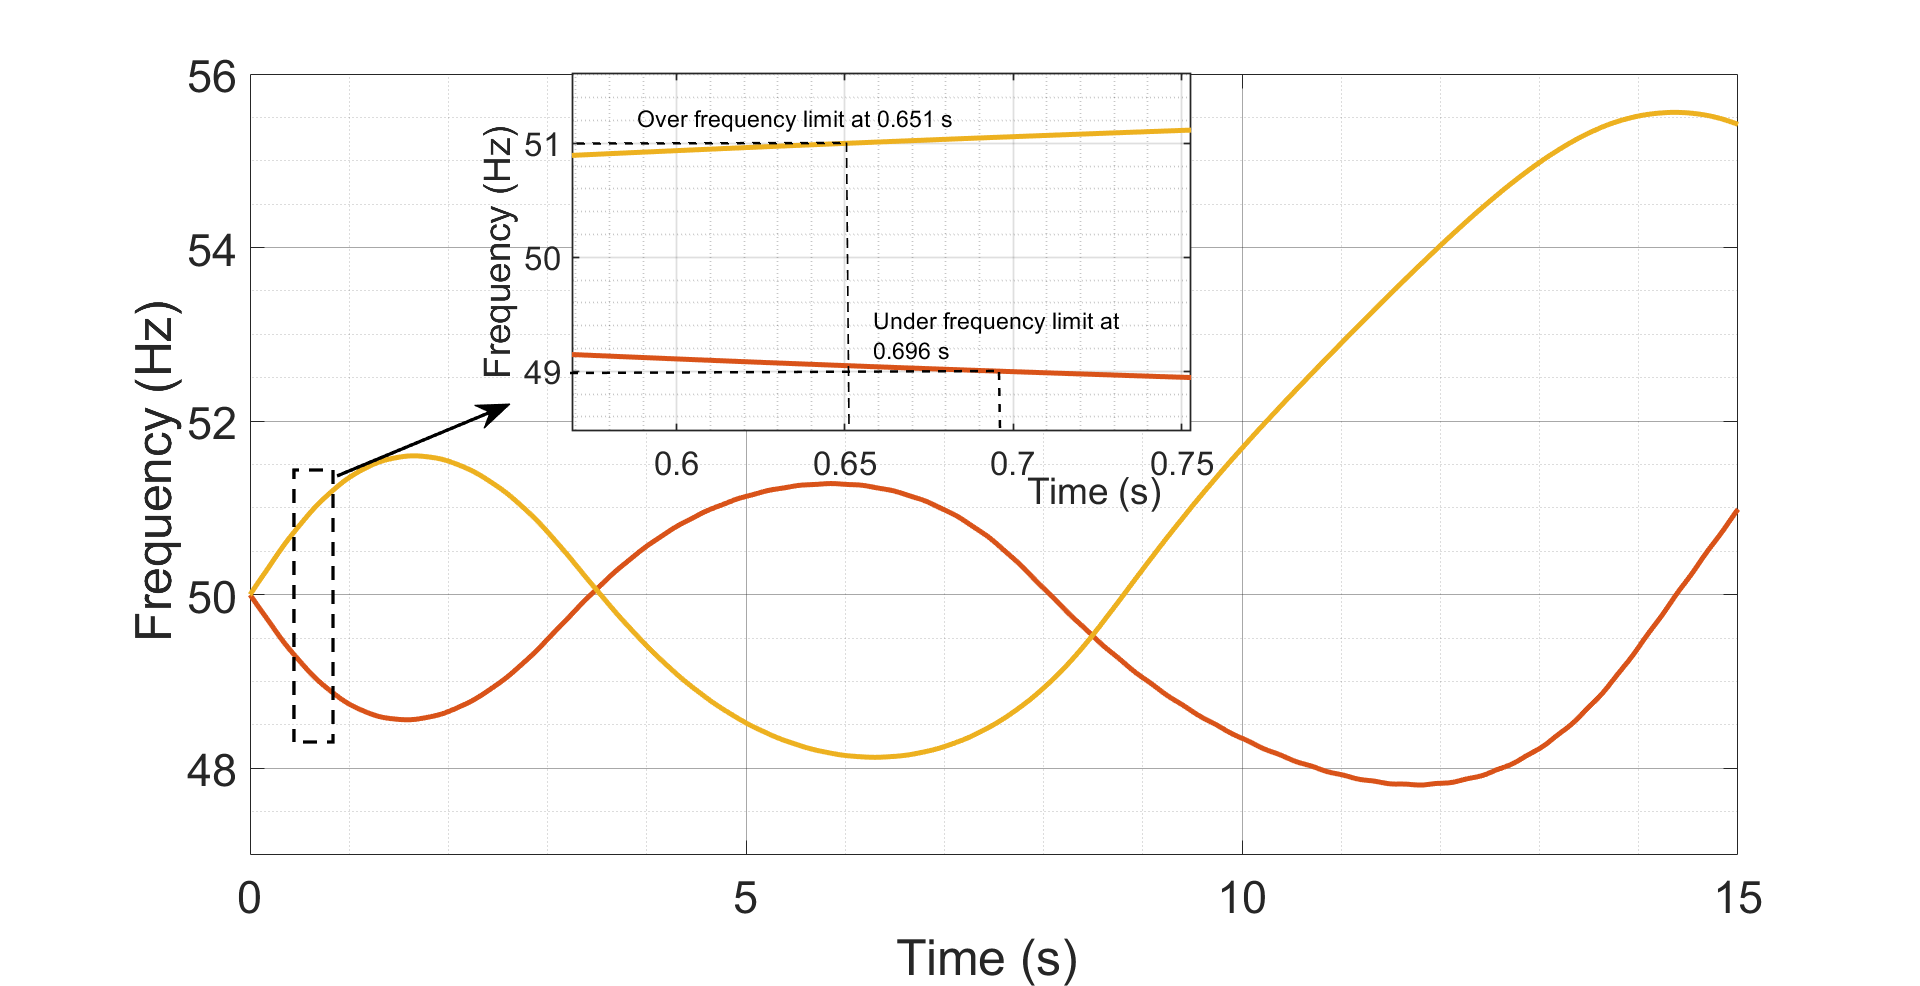
\includegraphics[width=0.75\textwidth]{/result/over_under}
	\caption{Under and over-frequency events in the extended IEEE model, a difference of 45 ms between each critical time is found.}
	\label{fig:res_over_under}
\end{figure}

In general, similar behavior is exhibit from the different models and approaches, even though they differ considerably in size and complexity. Hence, simplified block representation of the power system seems to be a fair way to sketch overall system trends and responses. The difference in critical time estimation between a full grid simulation and a simplified model was calculated to differ between 20-35\%, such difference could be crucial in fast power reserve studies and therefore should be considered when precise applications are implemented. A comprehensive method for estimation of the inverter based fast power reserve and critical time were developed and proved through the implementation in the two cases. 
